\documentclass{beamer}
\usepackage[utf8]{inputenc}

\usepackage{amsmath,amsfonts,amssymb,amsthm,
mathtools,mathrsfs}
\usepackage{physics}
\usepackage{xcolor}
\usepackage{hyperref}

\usepackage{tikz-cd} % arrow diagram

% Citation style
\usepackage[style=apa, backend=biber, natbib]{biblatex}
\addbibresource{../references.bib}

\usetheme{Madrid}
\usecolortheme{default}
\useoutertheme[subsection=false]{miniframes}
\setbeamertemplate{frametitle continuation}{}
\setbeamertemplate{bibliography item}[triangle]
\setbeamertemplate{sidebar right}{}
%\addtobeamertemplate{footnote}{}{\vspace{2ex}}

% Presenter notes
%\setbeameroption{show notes}



\title[Optimal Cryptoeconomic Policies]{Dynamic Modeling for Optimal Cryptoeconomic Policies}
\subtitle{Pitch Proposal Fall 2023}
\author{Mingxuan He}


\institute[UChicago]{
M.A. in Computational Social Science -- Economics\\
Department of Economics, University of Chicago\\
mingxuanh@uchicago.edu
}


\date{\today}


\begin{document}


% title page
\begin{frame}
\titlepage  
\end{frame}

% table of contents
% \begin{frame}
% \frametitle{Table of Contents}
% \tableofcontents
% \end{frame}


%----------------
\section{Introduction}

\begin{frame}{Research question}

\textbf{How should we design dynamic staking and burning policies for Proof-of-Stake cryptoeconomies?}\newline
\begin{itemize}
\item Current protocol-coded policies are static even though crypto-economies face dynamic shocks. ``Staking" and ``burning" rates are the primary coded policy rules in the underlying blockchain system
\begin{itemize}
    \item \textbf{Staking (increases ``token supply", decreases ``tokens in circulation")}: mint new tokens and give to those who stake their existing tokens as interest. Similar to interest on reserves.
    \item \textbf{Burning (decreases ``token supply")}: burn (remove from circulation) a portion of the transaction fee paid by users during blockchain transactions
    \end{itemize} \textbf{}
    
    \item Policy goal: maximize welfare for \underline{good actors}: users (increase in token price \& consumption) and validators (transaction fees)
\end{itemize}

\note{
shocks from the real economy: Banks failing, stock market, interest rates\\
shocks from other cryptoeconomies: Luna-Terra, FTX/Alameda
}

\end{frame}

%----------------
%\section{Literature Review}

\begin{frame}{Literature review}
    \begin{itemize}
        \item Micro foundations:\\
        {\footnotesize \textit{\citet{nisan2007algorithmic, budish2018economic, biais2019blockchain, gans2019more, gans2022mechanism, huberman2021monopoly}, etc.}}\\
        $\rightarrow$ \textbf{Block reward and transaction fee as incentive mechanisms}

        \item Pricing models of cryptocurrencies:\\
        {\footnotesize Bitcoin: \textit{\citet{athey2016bitcoin, garratt2018bitcoin, schilling2019some, schilling2019currency, catalini2020some, biais2023equilibrium, bolt2020value, hinzen2022bitcoin, chiu2017economics}, etc.}}\\
        {\footnotesize Proof-of-stake: \textit{\citet{catalini2020markets, saleh2019volatility, saleh2021blockchain}}}\\
        $\rightarrow$ \textbf{Static token supply means all shocks are absorbed by price}
        \item Monetary policies for stablecoins, platform tokens, and CBDCs:\\
        {\footnotesize \textit{\citet{cong2021tokenomics, cong2022token, cong2022staking, d2022can, fernandez2021central, zhu2019framework, sockin2023model, sockin2023decentralization}, etc.}}\\
        $\rightarrow$ \textbf{Optimizing policy for defending peg and/or making profit}
    \end{itemize}
\end{frame}

\begin{frame}{Contribution to the literature}
\begin{itemize}
    \item Practical: Most cryptoeconomic systems feature fixed-schedule token supply, creating highly volatile token prices
    \item Problem: Traditional models for optimal fiscal policy (e.g. Ramsey) and monetary policy (e.g. NK) are not directly transferrable to cryptoeconomies due to transaction fee role in the cryptoeconomy
    % \begin{itemize}
    %     \item deterministic token supply (Bitcoin\footnote{Satoshi Nakamoto (2008). Bitcoin: A peer-to-peer electronic cash system}), 
    %     fixed burn rate (Ethereum\footnote{Ethereum Documentation. ``Gas and Fees - Base fees"}), 
    %     naive dynamic burning (Binance Coin)
    % \end{itemize}
    \item Novel hypothesis: Dynamic token supply (via staking and burning policies) can be used to optimize welfare 
    \begin{itemize}
        \item implement in a dynamic equilibrium model framework
    \end{itemize}
\end{itemize}

\end{frame}





%----------------
\section{Model}
% \begin{frame}{Inspiration}
%     \begin{figure}
%         \includegraphics[width=0.75\textwidth]{biais_title.png}
%     \end{figure}
%     * Bitcoin's economic/consensus system (proof-of-work) is different from proof-of-stake
% \end{frame}


\begin{frame}{A model of proof-of-stake cryptoeconomies}
    \[
\begin{tikzcd}[ampersand replacement=\&, column sep = 4.5em, row sep = 4.5em]
Protocol 
\ar[d, shift right, "\substack{\text{newly minted}\\\text{tokens}\\(t+1)}" ']
\&
\ar[d, shift right, "\substack{\text{endow-}\\\text{ment}}" 'near start]
\ar[d, shift left, "\substack{\text{purchase}\\ \text{assets}}" near start]
\&
\ar[d, "\substack{\text{transact.}\\ \text{benefits}}" ]
\&
\\
Validators
\ar[u, shift right, red, "\substack{\text{stake}\\\text{tokens}\\(t)}" ' red ]
\& 
\substack{Young\\Users}
\ar[l,"\substack{\text{variable}\\ \text{fees (``tip")}}" ']
\ar[lu, red, "\substack{\text{base fees}\\ \text{(burned)}}" {sloped,auto}' red]
\ar[r, dashed, "t+1", 
"\substack{\text{hold}\\\text{assets}}" ']
\& 
\substack{Old\\Users}
\ar[r, "\substack{\text{hacked}\\ \text{tokens}}"]
\&
Hackers
\end{tikzcd}
\]

\begin{itemize}
    \item Inspired by Biais et al. (J Finance 2023) ``Equilibrium Bitcoin Pricing"
    \item Two-period OLG model
    \item Endogenous token supply (innovation over \citet{biais2023equilibrium})
    \item Assumption: Crypto's fundamental value comes from the stream of future transactional benefits\\
    \begin{itemize}
        \item e.g. access to unique goods, not expropriated/taxed/constrained by government, direct internet access
    \end{itemize}
\end{itemize}

\end{frame}


\begin{frame}{User's problem}
    \begin{itemize}
    \item Period t: allocates endowment income $e_t^u$ into three asset classes: risk-free $s_t$, crypto $q_t$, and fiat $\hat{q}_t$. To buy crypto they pay a two-part transaction fee $\varphi_t^b$ (burned) and $\varphi_t^v$ (goes to validator)\\
    \item Period t+1: receive interest $r_t$, transactional benefits $\theta_{t+1}$, and hacking loss $h_{t+1}$\\
    \end{itemize}

    \begin{align}
    c_t^u &= e_t^u - s_t - (1+ \varphi_t^b+\varphi_t^v) q_t p_t - \hat{q}_t \hat{p}_t\\
    c_{t+1}^u &=  s_t (1+r_t) + (1-h_{t+1})(1+\theta_{t+1}) q_t p_{t+1} + \hat{q}_t \hat{p}_{t+1}
    \end{align}


\end{frame}


\begin{frame}{Validator's problem}
    \begin{itemize}
        \item Period t: receive transaction fees $\varphi_t^v$, stake $L_t$
        \item Period t+1: receive staking yield $\delta_t$
    \end{itemize}
    \textbf{Trade-off:}
    \[
    \text{more staking at } t \Rightarrow
    \begin{cases}
        \text{more staking yield at } t+1\\
        \text{less circulating supply} \Rightarrow \text{less transact. fees at } t
    \end{cases}
    \]
    \begin{align}
    c_t^v &= e_t^v + \varphi_t^v q_t p_t - L_t p_t \\
    c_{t+1}^v &= (1+\delta_t) L_t p_{t+1} 
    \end{align}
\end{frame}


\begin{frame}{Token supply}
    \begin{align}
        M_{t+1} &= (M_t - L_t) + L_t (1 + \delta_t) - \varphi_t^b X_t \nonumber \\
        &= M_t + \delta_t L_t - \varphi_t^b X_t
    \end{align}
    $M_t$: total token supply\\
    $X_t \equiv M_t - L_t$: circulating supply \\
    \quad $\Rightarrow$ Token market clearing condition is $X_t=q_t$\\
    \ \\
    $^*$ In reality the total reward is $\delta_t L_t^\alpha$, with pre-set $\alpha\in [0,1]$\footnote{$\alpha=0.5$ for Ethereum. See Ethereum Documentation. ``Proof-of-Stake Rewards and Penalties"}. Here I set $\alpha=1$ for simplicity.
    % calculations: https://blog.bitmex.com/ethereums-proof-of-stake-system-calculating-penalties-rewards/
\end{frame}


\begin{frame}{First order conditions}    
    $^*$ using a deterministic version of the model
    \bigskip

    User's Euler equations:
    \begin{equation}
        \frac{u'(c_t^u)}{u'(c_{t+1}^u)} = \beta (1+r_t) 
        = \beta \frac{(1+\theta_{t+1})(1-h_{t+1})}{1+\varphi_t^b+\varphi_t^v} \frac{p_{t+1}}{p_t}
        = \beta \frac{\hat{p}_{t+1}}{\hat{p}_t}
    \end{equation}

    Validator's Euler equation:
    \begin{equation}
        \frac{u'(c_t^v)}{u'(c_{t+1}^v)} = \beta (1+\delta_t) \frac{p_{t+1}}{p_t}
    \end{equation}

    %WIP: Equilibrium solutions with stochasticity \& log/CRRA preferences
\end{frame}

\begin{frame}{Token market equilibrium}
    \hyperlink{det_math}{\beamerbutton{Appendix: deterministic math}}
    \begin{figure}
        \centering
        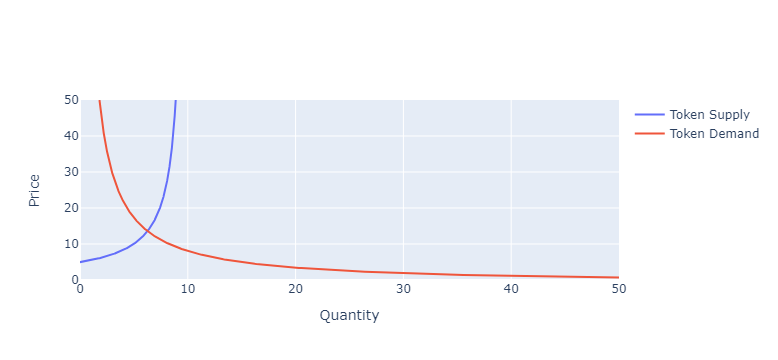
\includegraphics[width=\textwidth]{../Figures/det_SD.png}
        \caption{Illustration of token market equilibrium using artificial parameters. Both supply and demand are convex in $q$}
    \end{figure}
    
\end{frame}

%----------------
\section{Calibration}

\begin{frame}{The Ethereum (ETH) blockchain}
    Ethereum (created by V. Buterin in 2013) is currently the second largest cryptoeconomy after Bitcoin.\\
    \bigskip
    Important historical upgrades to Ethereum's tokenomics:
    \begin{itemize}
        \item London upgrade (Aug 2021): introduced base fee burning via EIP-1559
        \item ``The Merge" (Sep 2022): transition from computing-based (PoW) to staking-based issuance (PoS) i.e. Ethereum 2.0
        \item Shanghai-Capella upgrade (Apr 2023): unlocked withdrawls of staked ETH \footnote{Hypothesis: this changes validators' staking behaviors}
    \end{itemize}
\end{frame}

\begin{frame}{Ethereum 2.0 data}
    Despite having only 6-12 months of history, Ethereum 2.0 data is rich and highly accessible:
    \begin{itemize}
        \item All transactions are publicly broadcasted to the blockchain every 12 seconds (block time), 24/7
        \item All validators' staking actions and rewards are also recorded
        \item ETH-USD price data are available from both onchain sources (DEX) and offchain (CEX/``oracle") sources
    \end{itemize}

\end{frame}

\begin{frame}{Features for calibration}
    \begin{itemize}
        \item Method: baseline - OLS; advanced - VAR
        \item Data sources: Ethereum prices from Messari API, txn fees from Dune Analytics, staking data from beaconcha.in
        \item Proxy for transactional benefits/convenience yields: 
        \begin{itemize}
            \item Throughput measures: average onchain txn processing per second \citep{cong2022staking}; user operations per second (new measure proposed by industry researchers)
            \item Network-based measures: Metcalfe's measure $\log(DailyActiveAddresses^2)$; 
            \item Additional controls: \href{https://www.ncsl.org/financial-services/cryptocurrency-2023-legislation}{index on US crypto regulation (NCSL.org)}
        \end{itemize}
        \item Proxy for hacking: manually index major hacks and wallet losses (problem: frequency is much lower than txn/staking actions)
    \end{itemize}
\end{frame}

% \begin{frame}{More extensions to model \& estimation}

% \begin{enumerate}
%     \item Modify validators' budget constraint: incorporates costs of validation under PoS and PoW \parencite{biais2019blockchain, saleh2019volatility, saleh2021blockchain}
%     \item Improvement in model calibration 
%     \begin{itemize}
%         \item novel time series data on Ethereum price and transaction fees
%         \item estimate transactional benefits using the NVT (network value to transaction ratio) or RVT (realized value to transaction ratio) metric instead of event-based index
%     \end{itemize}
%     \item Use vector autoregression models for exogenous process in variable transaction fees and transaction benefit (e.g. sign restrictions)
% \end{enumerate}
% \end{frame}


% \begin{frame}{Proposed Project Timeline}
% \begin{itemize}
%     \item Spring '23: As final project for ECMA33603 (Macro \& Financial Frictions), replicate the baseline model and implement extensions part 1 (endogenous token supply)
%     \item Summer '23: Implement extensions part 2; gather ideas from industry internship in Ethereum research \& dev
%     \item Fall '23 - Winter '24: Extensions part 3: Data collection, model calibration (likely using Ethereum data)
%     \item Spring '24: Finish paper
% \end{itemize}
% \end{frame}


% -----------------
\section*{}
\begin{frame}[allowframebreaks, noframenumbering]{References}
    %\nocite{*}
    %\bibliographystyle{apalike}
    %\bibliography{references}
    \printbibliography
\end{frame}


\section{Appendix}
\begin{frame}[noframenumbering]{Deterministic solutions (cont.)}
    \label{det_math}
    \begin{align}
        \intertext{Inverse demand curve:}
        q_t &= \left[ \beta \frac{e_t^u}{p_t} - (1+\beta)m_t \frac{\hat{p}_t}{p_t} \right] \cdot\\
            & \left[\beta(1+ \varphi_t^b+\varphi_t^v) + \frac{(1-h_{t+1})(1+\theta_{t+1})}{1+r_t} \frac{p_{t+1}}{p_t}\right]^{-1}\\
        \intertext{Inverse supply curve:}
        q_t &= \left(1+\frac{\beta}{1+\beta}\varphi_t^v\right)^{-1} \left(M_t - \frac{\beta}{1+\beta}\frac{e_t^v}{p_t}\right)
    \end{align}
    
\end{frame}

\begin{frame}[noframenumbering]{Deterministic solutions (cont.)}
    \begin{align}
        \intertext{Token market clearing implies $\frac{1}{p_t^*}$ must satisfy the quadratic equation}
        A_t \frac{1}{p_t^*} &= (M_t + B_t\frac{1}{p_t^*}) (C_t + D_t\frac{1}{p_t^*}) \\
        \intertext{where}
        A_t &:= \left[ \beta e_t^u - (1+\beta)m_t \hat{p}_t \right] \left(1+\frac{\beta}{1+\beta}\varphi_t^v\right);\quad
        B_t := - \frac{\beta}{1+\beta} e_t^v;\\
        C_t &:= \beta(1+ \varphi_t^b+\varphi_t^v);\quad
        D_t := \frac{(1-h_{t+1})(1+\theta_{t+1})}{1+r_t} p_{t+1}
        \end{align}
\end{frame}

\begin{frame}[noframenumbering]{Deterministic solutions (cont.)}
    \begin{align}
        \intertext{Therefore the closed-form solution for equilibrium token price is given by}
        p_t^* &= \frac{2B_tD_t}{A_t-M_t D_t-B_tC_t - \sqrt{(M_t D_t+B_t C_t-A_t)^2-4M_t B_tC_tD_t}}\\
        \intertext{under some technical conditions.}\nonumber
    \end{align}
    
\end{frame}

\end{document}
